\documentclass[10pt, a4paper]{amsart}
\usepackage{graphicx}
\usepackage{hyperref}
\usepackage[english]{babel}
\usepackage{setspace}
\usepackage{cleveref}
\usepackage{physics}
\usepackage{appendix}
\usepackage{listings}
\usepackage{pgfplotstable, booktabs, mathpazo}
\usepackage[T1]{fontenc}
\usepackage{color}
\usepackage{amssymb}
\usepackage{float}
\usepackage[export]{adjustbox} % loads also graphicx
\usepackage{etoolbox}
\usepackage{datetime}
\usepackage{gensymb}
\usepackage{esvect}
\usepackage{caption}
\usepackage{subcaption}

\setlength{\parskip}{0.5em}
\setlength{\parindent}{0em}
\renewcommand{\arraystretch}{1.25}
\setlength{\tabcolsep}{8pt}
\setcounter{tocdepth}{1} % choose only to show sections in toc
%\everymath{\displaystyle}

\makeatletter
\patchcmd{\@maketitle}
  {\ifx\@empty\@dedicatory}
  {\ifx\@empty\@date \else {\vskip3ex \centering\footnotesize\@date\par\vskip1ex}\fi
   \ifx\@empty\@dedicatory}
  {}{}
\patchcmd{\@adminfootnotes}
  {\ifx\@empty\@date\else \@footnotetext{\@setdate}\fi}
  {}{}{}
\makeatother

\renewcommand{\r}{\right}
\renewcommand{\l}{\left}
\captionsetup{width=\linewidth}
\captionsetup{belowskip=10pt}

\definecolor{mygreen}{rgb}{0,0.6,0}
\definecolor{mygray}{rgb}{0.5,0.5,0.5}
\definecolor{mymauve}{rgb}{0.58,0,0.82}
\definecolor{lgray}{gray}{0.95} 

\lstset{
  backgroundcolor=\color{lgray},   % choose the background color; you must add \usepackage{color} or \usepackage{xcolor}
  basicstyle=\footnotesize,        % the size of the fonts that are used for the code
  breakatwhitespace=false,         % sets if automatic breaks should only happen at whitespace
  breaklines=true,                 % sets automatic line breaking
  captionpos=b,                    % sets the caption-position to bottom
  commentstyle=\color{mygreen},    % comment style
  deletekeywords={...},            % if you want to delete keywords from the given language
  escapeinside={\%*}{*)},          % if you want to add LaTeX within your code
  extendedchars=true,              % lets you use non-ASCII characters; for 8-bits encodings only, does not work with UTF-8
  keepspaces=true,                 % keeps spaces in text, useful for keeping indentation of code (possibly needs columns=flexible)
  keywordstyle=\color{blue},       % keyword style
  language=c++,
  otherkeywords={*,...},           % if you want to add more keywords to the set
  rulecolor=\color{black},         % if not set, the frame-color may be changed on line-breaks within not-black text (e.g. comments (green here))
  showspaces=false,                % show spaces everywhere adding particular underscores; it overrides 'showstringspaces'
  showstringspaces=false,          % underline spaces within strings only
  showtabs=false,                  % show tabs within strings adding particular underscores
  stepnumber=2,                    % the step between two line-numbers. If it's 1, each line will be numbered
  %stringstyle=\color{mymauve},     % string literal style
  tabsize=2,	                   % sets default tabsize to 2 spaces
}

\title[NTNU: porous media]{NTNU: porous media\\\hrulefill\;\;FYS4420\;\;\hrulefill\\
Experimental techniques in Condensed Matter physics}

\author[Foschi, Sigorini \& Slongo]{Marianna Foschi, Stefano Sigorini and Francesco Slongo}
\date{\today} 

\begin{document}

\onehalfspacing

\begin{titlepage}
\begin{abstract}
    In this paper we are presenting the measurements of porosity and permeability of a core sample of sandstone. The analysis is aimed at studying the oil recovery from the rock. The porosity was measured with a Helium porosimeter and with the saturation technique, while the permeability was estimated using both a permeameter and flow of nitrogen through the sample. The two values of porosity are $\simeq0.215$ and $\simeq0.223$. They result different because of a systematic error. The two values of permeability ($\simeq 200\;mD$ and $\simeq620\;mD$) cannot be compared because they are measured in different conditions. Lastly, we saturated the sample with oil and performed drainage with water and water with soap, to measure how much oil could be extracted. In total, we were able to extract $63.3\%$ of the initial amount of oil.
\end{abstract}
\maketitle
\end{titlepage}

\section{Introduction}

An important aim of reservoir engineering is to estimate how much oil can be extracted from the reservoir and to study which techniques grant the highest recovery. For this purpose, it is fundamental to study the porosity of the rock that composes the reservoir, its absolute and relative permeability (for a given fluid) and the fluids contained in it. Samples collected from the reservoir by drilling or coring are usually used for this purpose.

We analysed a cylindrical sample of sandstone. To estimate porosity, we performed measurements of the pores volume, first using the Helium technique and then the saturation technique. We used two different approaches to measure permeability: firstly using nitrogen and secondly with a porosimeter. At last we performed drainage of the sample that was saturated with oil and water. We used water and water with soap as displacing fluids.

In \cref{sec:theory} we shall briefly explain the theory, introducing some notions. In \cref{sec:methods} we shall give details of the experimental procedure and setup, while in \cref{sec:resdisc} we will present and explain our results.

\section{Theory}\label{sec:theory}

\subsection{Porosity}
The porosity $\phi$ of a rock is defined as the ratio between the volume of the pores and the bulk volume:
\begin{equation}\label{eq:Poro}
    \Phi = \frac{V_p}{V_b}
\end{equation}
To be more precise, we can define two different types of porosity: \textit{total porosity}, where $V_p$ consists of all the pores, and \textit{effective porosity}, where $V_p$ considers only the interconnected pores. In the case of drainage, we are only concerned about the effective porosity so, from now on, we will refer to that only. Porosity depends on the following properties of the rock:
\begin{description}
    \item [$\bullet$ grain shape] the more the grains are spherical, the more they can be packed tightly and the less is the porosity;
    \item [$\bullet$ sorting] if the rock contains grains of many different sizes, the empty spaces are better filled, so the porosity is lower;
    \item [$\bullet$ packing] grains can be positioned more or less compactly, corresponding to a lower or higher porosity.
\end{description}
A way to calculate the porosity is to compute the bulk volume $V_b$ (e.g. by measuring the height $h$ and the diameter $d$ of the cylindrical sample) and the pore volume $V_p$ (e.g. with the Helium technique). Using a Helium porosimeter, it is possible to measure the volume of helium that fills the pores. Helium is used because its molecules are small and they can quickly permeate all the pores, it is close to an ideal gas and it is unlikely to react with any substance in the rock. 

Another way to determine the pore volume is to saturate the sample with a liquid of known density $\rho$ and measure the sample's increase in weight, so to obtain:
\begin{equation}
    V_p = \frac{m_2 - m_1}{\rho}
\end{equation}
where $m_1$ is the mass of the dry sample and $m_2$ the one after saturation.

\subsection{Permeability}\label{sec:theory:perm}
\textit{Absolute permeability} measures the capacity of rock to transmit fluid when a single fluid saturates the pores. Absolute permeability $k$ can be calculated from Darcy's law for incompressible fluids:
\begin{equation}
    \label{e:darcy}
    k = \frac{q \mu L}{A \Delta P}
\end{equation}
where $q$ is the volumetric flow rate, $A$ is the cross section, $\mu$ is the permeability, $L$ is the length and $\Delta P \equiv P_2 - P_1$ is the pressure difference between the object's ends. Permeability is measured in darcy $1 D = 1 \, \mu m^2$.

The permeability of a rock sample can be measured by allowing a liquid (of known viscosity) to flow through the sample (of known dimensions) and measuring the flow rate and the pressure drop. As an alternative, a gas can be used instead of a liquid, but in this case Darcy's law must be modified to account for the compressibility of the gas:
\begin{equation}
    k = \frac{2 P_a q \mu L}{A (P_2^2 - P_1^2)}
\end{equation}
where $P_a$ is the atmospheric pressure. Experimental results show that measuring absolute permeability with a gas results in it to be a function of the gas mean pressure and it differs from gas to gas. Conversely, it should depend only on the rock properties.

This can be explained by the so-called \textit{Klinkenberg effect}. It is due to gas slippage, which happens when the diameters of the capillary openings are of the same order of the mean free path of the gas. The latter is determined by the molecular size, hence the dependence of $k$ on the type of gas and on kinetic energy (which depends itself on temperature and pressure). The relation between the apparent permeability $k_a$ for a gas at pressure $P_m$ and the true permeability $k_L$ measured with a liquid is:
\begin{equation}\label{eq:Klink}
    k_a = k_L \left( 1 + \frac{b}{P_m}\right)
\end{equation}
where $b$ is known as the \textit{Klinkenberg factor}, defined as $b = C/r$, $r$ is the average pore radius and $C$ is a gas-dependent constant.

\subsection{Relative Permeability}
Absolute permeability is useful when only one fluid saturates the porous medium. If more than one fluid flows through the material, the notions of \textit{effective permeability} and \textit{relative permeability} must be introduced. The former is the medium's capacity to conduct a fluid when saturation is lower then the volume of all the pores. The latter is the ratio between effective permeability and absolute permeability. Consequently, the relative permeability of a fluid is given by:
\begin{equation}
    k_\mathrm{rel} = \frac{Q_0\;\mu_0\;L}{k\;\Delta P\;A}
\end{equation}
where $L$ is the length of the sample, $A$ is the cross section area, $\Delta P$ is the pressure difference between the sample's ends, $\mu$ is the fluid's viscosity, $Q$ the volumetric flow rate of the fluid and $k$ the absolute permeability. 

\section{Methods}\label{sec:methods}
The aim of this section is to describe the experiments we performed at the NTNU didactic laboratory. We studied a porous medium sample and thanks to different experiments and instruments we computed its porosity, permeability and other relevant parameters.

\subsection{Porosity measurement}
To begin with, we measured the sample's diameter with a caliper, so that to calculate its volume. This shall be used to estimate the porosity. Moreover, we weighted the sample.
\begin{figure}[H]
    \centering
    \begin{minipage}{0.45\textwidth}
        In order to estimate the porosity of the sample, we measured the pores volume using a so-called \textit{Helium porosimeter}. The apparatus is shown in \cref{f:porosimeter}. We first placed the sample inside the cylinder and then put it in place to start the measurement. We allowed He to flow from the tank and set the pressure to $15\;bar$. Then we configured the porosimeter and began the procedure. The big hand (see \cref{f:porosimeter}) reported the volume of gas that had flowed into the medium. We also performed a measurement with the empty cylinder so that to estimate its own (internal) volume.
    \end{minipage}\hfill
    \begin{minipage}{0.5\textwidth}\centering
        \includegraphics[width=\textwidth]{porosimeter.jpeg}
        \caption{Helium porosimeter. In the foreground is the cylinder inside which we put the sample.}
        \label{f:porosimeter}
    \end{minipage}
\end{figure}

\subsection{Permeability measurements}
We estimated permeability using two different techniques.

The first method used the apparatus shown in \cref{f:perm1}. The sample was put into the white plastic cylinder. Water flow inside the sink allowed to create vacuum between the cylinder internal walls and the gasket, so that to allow the sample to be inserted. Then the vacuum creator was stopped and the cylinder closed with the cap shown
in \cref{f:perm1_detail}. The system was connected to a tank of nitrogen. After closing the cap, nitrogen was allowed to flow out of the container at a pressure of $15\;bar$. The pressure given by nitrogen was made also sure the gasket was in contact with the sample. So, during the experiment, we avoided the gas to leak from the edges of the gasket and instead it went through the sample. Then, thanks to the two black knobs shown in \cref{f:perm1} (highlighted in the light blue circles), the flow of nitrogen was regulated so that to have two given values of pressure at the two ends of the white cylinder. The pressure could be read thanks to the two red displays (highlighted in yellow). During the measurements, we increased the pressure, keeping the difference constant, and for all these we registered the values of the flow rate displayed by a gauge at the end of the tubing.

\begin{figure}[!h]
    \centering
    \begin{minipage}{0.8\textwidth}
        \includegraphics[width=\textwidth]{perm1_2.jpeg}
        \subcaption{Apparatus.}
        \label{f:perm1}
    \end{minipage}\hfill
    \begin{minipage}{0.2\textwidth}
        \centering
        \includegraphics[angle=90,width=0.9\textwidth]{perm1_1.jpeg}
        \subcaption{cap detail.}
        \label{f:perm1_detail}
    \end{minipage}
    \caption{First permeability measurement. The knobs highlighted in light blue were used to regulate pressure; the displays in yellow were used to read the pressure values.}
\end{figure}

The second method used the permeameter shown in \cref{f:perm2}.
The sample was put in the given cylinder connected to the machinery. For this task, the fluid used was air. Once the air flow from the tank was opened, again to a pressure of $15\;bar$, thanks to the black knob at the bottom-left corner of the permeameter (highlighted in the blue circle in \cref{f:perm2}), air was allowed into the cylinder. The system was configured (thanks to the knob highlighted in red) so that the pressure difference between the two ends of the sample was approx. $8\;mbar$. Then, a given software connected to the machinery processed the data and computed the permeability. The air pressure was also used to keep the gasket close to the sample, as in the previous measurements.

\begin{figure}[!h]
    \centering
    \begin{minipage}{0.5\textwidth}
        \includegraphics[width=0.9\textwidth]{perm2.jpg}
        \subcaption{Apparatus.}
        \label{f:perm2}
    \end{minipage}\hfill
    \begin{minipage}{0.5\textwidth}
        \includegraphics[width=\textwidth]{perm2_2.jpeg}
        \subcaption{Software for computing the permeability. Data were collected from the apparatus shown in \cref{f:perm2} and processed by a given software in order to estimate the permeability.}
        \label{f:perm2_detail}
    \end{minipage}
    \caption{Second permeability measurement.}
\end{figure}

\subsection{Saturation}
After completing the experiments in the morning, we put the sample in the glass container shown in \cref{f:essicatore}.

\begin{figure}[H]
    \centering
    \begin{minipage}{0.45\textwidth}
        Inside, vacuum was created thanks to a pump (connected via the tubing highlighted in light blue) and the sample was put into $3\%$ salt water. This last was put into the container from a pocket connected via the tubing highlighted in yellow.  We let this run for approximately one hour. This process saturates the porous medium with e.g. salt water. This is needed to run the following experiment, where we wish to determine the percentage of oil that can be extracted from the pores, given the initially introduced quantity.
    \end{minipage}\hfill
    \begin{minipage}{0.5\textwidth}
    \centering
        \includegraphics[width=\textwidth]{essicatore_det.jpeg}
        \caption{Glass container used for vacuum.}
    \label{f:essicatore}
    \end{minipage}
\end{figure}
Once saturation was completed, we weighted the sample again so that we could compute the mass different and therefore the porosity with a different technique.

\subsection{Oil-extraction experiment}
The last experiment was aimed at understanding how much oil could be extracted from the pores, given the initially introduced amount. The sample was placed into the white plastic cylinder (see \cref{f:lastexp}) and this last was sealed. First, the tubing was connected to a $3\%$ salt water tank and the flow into the cylinder started. The flow rate was set to $5\;ml/min$ during all the following tasks. The flow out of it (red end in \cref{f:lastexp}) was conveyed into a glass flask. This way, we made sure that the system was saturated (as much as possible) with the saline water. Second, we connected the tubing to an oil container and allowed the flow. We kept the flow active until oil began to appear in the output flow. At that point, we could assume it had displaced the maximum possible amount of water. Then, we re-configured the system with the salt water tank. The output flow was now collected into test tubes, so that to be able to measure the amount of oil displaced by water. Finally, when the output was mainly composed of water, we connected the system to a third tank containing water with soap (in a $1\%$ concentration). Here, we wished to observe the surfactant behaviour of soap. Indeed, we were able to extract a bit more oil.

\begin{figure}[H]
    \centering
    \includegraphics[width=\textwidth]{lastexp.jpeg}
    \caption{Experimental setup for oil extraction task. The flow direction was from the end highlighted in yellow to the one in red.}
    \label{f:lastexp}
\end{figure}

\section{Results and Discussion}\label{sec:resdisc}
\subsection{Porosity}
In this part of the analysis we shall consider both our sample and the one studied by the other group. In this way, we will be able to compare the results and discuss them in a more complete way. In order to calculate the porosity of the cores, let us first compute their total volume. We shall refer to the height of the cores as $h$, their diameter as $d$ and their cross-section area as $A$. Starting from these, the total volume can be computed using the cores size:
\begin{equation}
    V_{tot} = \frac{\pi d^2 h}{4}
\end{equation}
Since we are interested in the pores volume, we measure the volume of a container filled with helium with the core ($V_1$) and without ($V_2$). These values are presented in \cref{tab:CorDim}.
\begin{table}[H]
    \centering
    \begin{tabular}{ccc}
    \toprule
        Parameter & Core 1 & Core 2 \\
    \midrule
        $h \,[cm]$ & $4.0660 \pm 0.0003$ & $4.0510 \pm 0.0003$ \\
        $d \,[cm]$ & $3.7780 \pm 0.0003$ & $3.7700 \pm 0.0003$ \\
        $A \, [cm^2]$ & $11.210 \pm 0.002$ & $11.162 \pm 0.002$ \\
        $V_{tot} \,[cm^3]$ & $45.580 \pm 0.010$ & $45.220 \pm 0.008$ \\
        $V_1\,[cm^3]$ & $58.00 \pm 0.03$ & $57.50 \pm 0.03$\\
        $V_2\,[cm^3]$ & $22.90 \pm 0.03$ & $22.00 \pm 0.03$\\
    \bottomrule
    \end{tabular}
    \caption{Parameters of the cores. The error on the values is the reading one (or propagated from it).}
    \label{tab:CorDim}
\end{table}
The difference between $V_1$ and $V_2$ is the volume of rock (excluding pores) in the cores:
\begin{equation}
    V_{rock} = V_1 - V_2
\end{equation}
Finally, from the difference between the total volume and the rock volume, we get the volume of the pores:
\begin{equation}
    V_{pores} = V_{tot} - V_{rock}
\end{equation}
We can compute the porosity of the cores with \cref{eq:Poro}. The values are presented in \cref{tab:CorVol}.
\begin{table}[H]
    \centering
    \begin{tabular}{ccc}
    \toprule
        Parameter & Core 1 & Core 2 \\
    \midrule
        $V_{rock} \,[cm^3]$ & $35.10 \pm 0.04$ & $35.50 \pm 0.04$ \\
        $V_{p} \, [cm^3]$ & $10.48 \pm 0.04$ & $9.72 \pm 0.04$ \\
        $\phi$ & $0.2299 \pm 0.0008$ & $0.2150 \pm 0.0010$\\
    \bottomrule
    \end{tabular}
    \caption{Computed values of volumes and porosity. The uncertainties was propagated from those on the parameters in \cref{tab:CorDim}.}
    \label{tab:CorVol}
\end{table}
From \cref{tab:CorVol} we see that the first core has a higher porosity than the second one. We expect the first core to be able to contain more water/oil per unit of bulk volume.

We can proceed in another way to obtain the effective porosity. We begin measuring the mass of the dry cores, so as to compute the mass of the rock. After saturating the cores with some fluid, we re-measure the mass and therefore compute the difference with respect to the dry values. Using the fluid's own density, one can calculate the volume of the pores (see \cref{tab:CorMasses}). The fluid's density is estimated using the following measured values\footnote{The uncertainties are the reading one. The bottle volume value is written with no error as this is negligible.}:
\begin{align}
     V_{bottle}&=50.42\;cm^3\nonumber\\ m_{water}&=51.3580 \pm 0.0003\;g\nonumber\\ \rho_{water}&=1.018604 \pm 0.000006\;g/cm^3
\end{align}
\begin{table}[H]
    \centering
    \begin{tabular}{ccc}
    \toprule
        Parameter & Core 1 & Core 2\\
    \midrule
        $m_{dry} \, [g]$ & $90.7530 \pm 0.0003$ & $93.0440 \pm 0.0003$ \\
        $m_{wet} \, [g]$ & $101.5880 \pm 0.0003$ & $103.3160 \pm 0.0003$ \\
        $V_{p} \, [g]$ & $10.6371 \pm 0.0004$ & $10.0844 \pm 0.0004$ \\
        $\phi$ & $0.23337\pm0.00004$ & $0.22301\pm0.00004$ \\
    \bottomrule
    \end{tabular}
    \caption{Second method to estimate porosity. The uncertainties are reading one or propagated opportunely.}
    \label{tab:CorMasses}
\end{table}
Comparing the values of porosity in \cref{tab:CorMasses,tab:CorVol}, we observe that the latter ones are slightly higher then the former.

We can explain the fact that with the saturation technique we get a higher value of the porosity with a systematic error due to the presence of some water drops on the scale.

\subsection{Permeability}
Henceforth, we shall just consider our sample. Following, we wish to compute the permeability of the core. We carried it out in two ways.

First, we measure the flow rate of nitrogen through the core. The viscosity of nitrogen is:
\begin{equation}
    \mu = 0.0179\;cp=0.0179\;mPa\,s
\end{equation}
The measurements of the flow rate result in the following data (\cref{tab:CorPres}):
\begin{table}[H]
    \centering
    \begin{tabular}{ccc}
    \toprule
        $P_1 \, [bar]$ & $P_2 \, [bar]$ & $Q[L/min]$ \\
    \midrule
        $1.20 \pm 0.03$ & $1.00 \pm 0.03$ & $1.000 \pm 0.003$ \\
        $1.30 \pm 0.03$ & $1.10 \pm 0.03$ & $1.060 \pm 0.003$\\
        $1.40 \pm 0.03$ & $1.20 \pm 0.03$ & $1.120 \pm 0.003$\\
        $1.50 \pm 0.03$ & $1.30 \pm 0.03$ & $1.170 \pm 0.003$\\
    \bottomrule
    \end{tabular}
    \caption{Pressures and flow rates for the calculus of the permeability. The uncertainty on the values is the reading error.}
    \label{tab:CorPres}
\end{table}
Through Darcy's law (see \cref{e:darcy}) we obtain the apparent permeability values reported in \cref{tab:perm}.
\begin{table}[H]
    \centering
    \begin{tabular}{cc}
    \toprule
        $P_m \, [bar]$ & $k_a \, [D]$ \\
    \midrule
        $1.10 \pm 0.02$ & $0.492 \pm 0.002$ \\
        $1.20 \pm 0.02$ & $0.4780 \pm 0.0014$\\
        $1.30 \pm 0.02$ & $0.4660 \pm 0.0013$\\
        $1.40 \pm 0.02$ & $0.4520 \pm 0.0012$\\
    \bottomrule
    \end{tabular}
    \caption{Apparent permeability. The uncertainty on the values are propagated from the previous measures.}
    \label{tab:perm}
\end{table}
In the calculation of the error of $k_a$ we do not consider the error on the pressures $P_1$ and $P_2$. We do this because we suppose that the fluctuations on the pressures are way lower than the resolution error. In this way, when lately we will perform a least squares linear regression (with the $\chi^2$ as cost function).
As explained in \cref{sec:theory:perm}, when using a gas the permeability turns out to be dependent on the average value of pressure. This can be observed in \cref{fig:Trend2}. 
\begin{figure}[H]
    \centering
    \includegraphics[width=\textwidth]{Trend_Core1.eps}
    \caption{Apparent permeability $k_a$ as a function of $P_m$.}
    \label{fig:Trend2}
\end{figure}
The trends in \cref{fig:Trend2} is the one we expected: as $P_m$ increases, the apparent permeability decreases.

Indeed we previously obtained the apparent permeability $k_a$. To obtain the permeability of a liquid we take into consideration the Klinkenberg effect. To begin with, we plot the values of apparent permeability $k_a$ against $1/P_m$ (see \cref{fig:Fit_Core2}).
\begin{figure}[H]
    \centering
    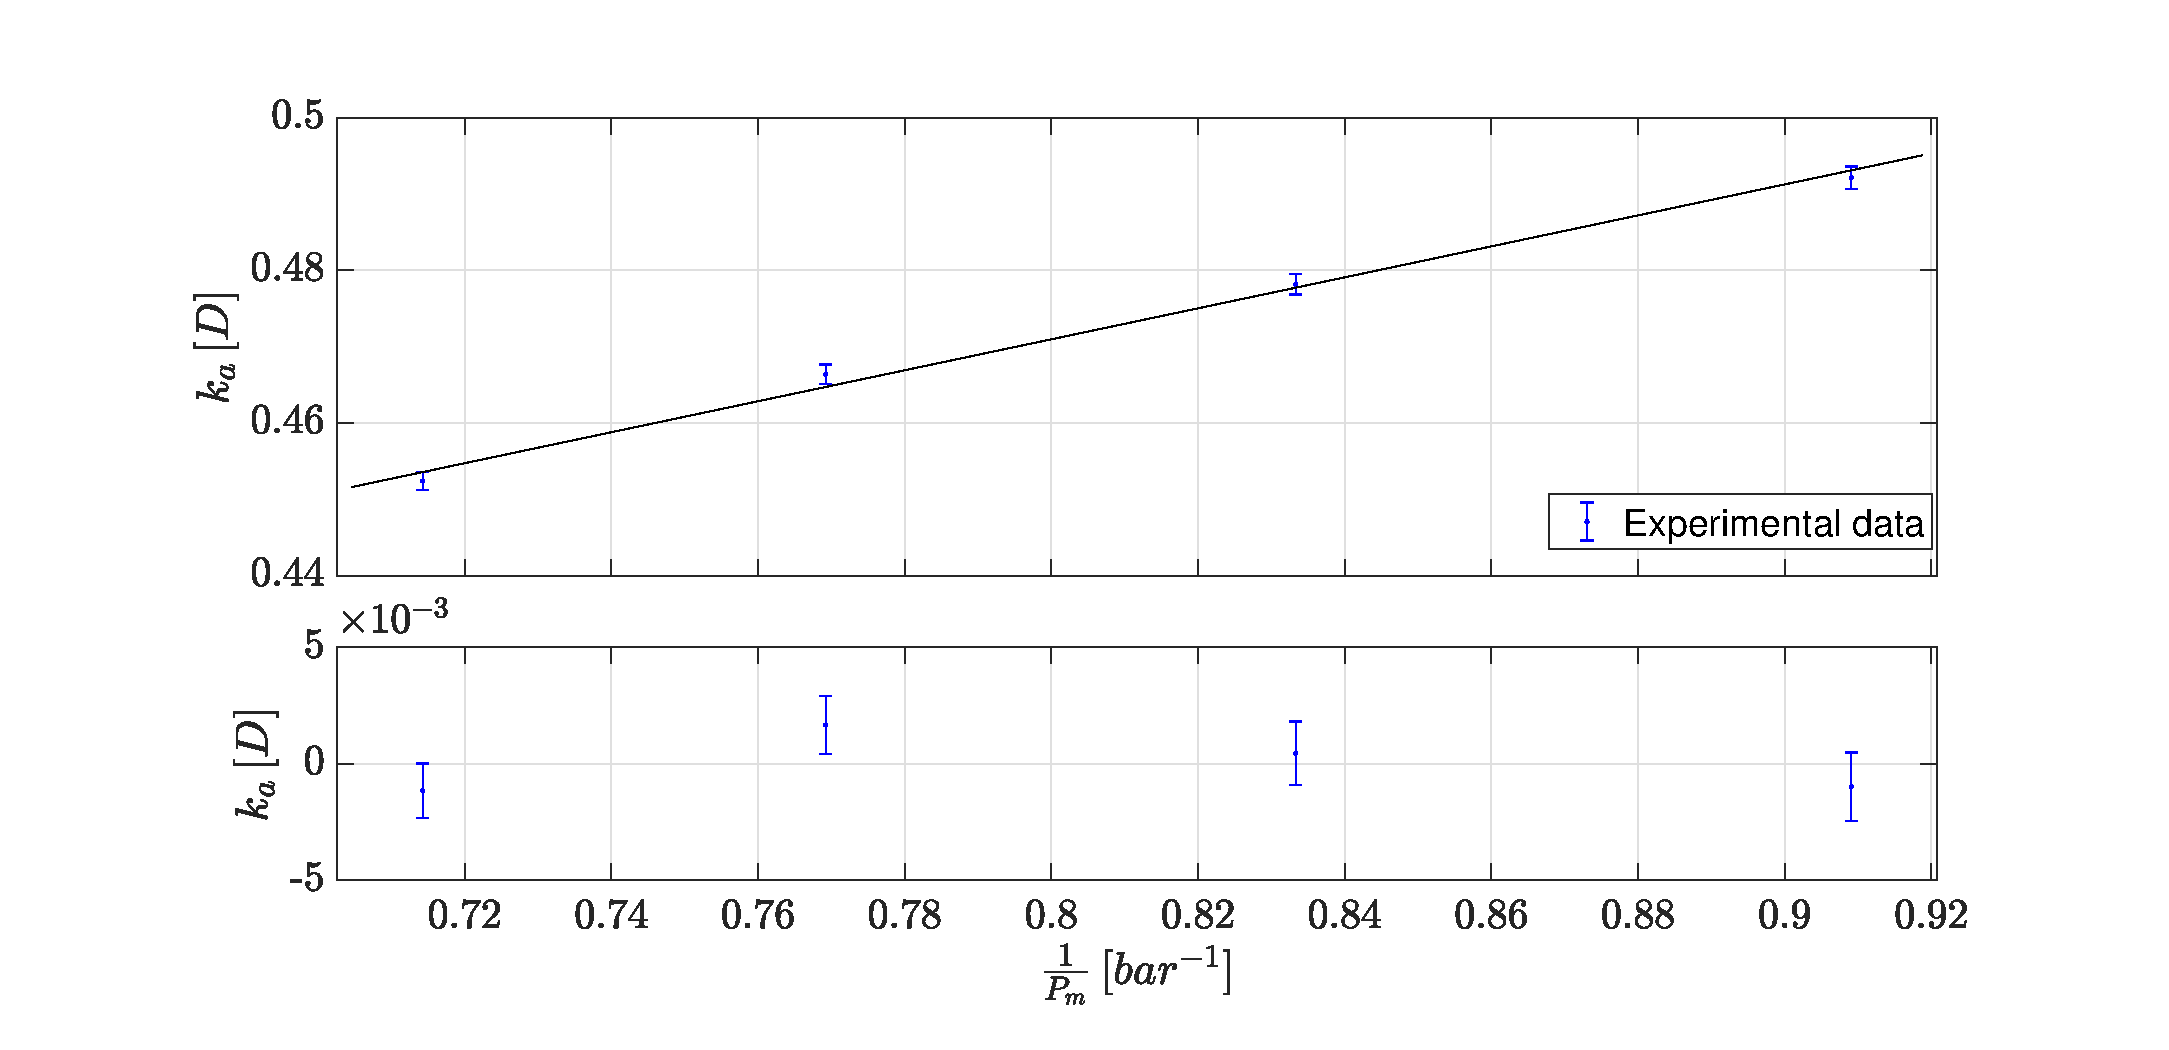
\includegraphics[width=\textwidth]{Fit_Core2.eps}
    \caption{Apparent permeability as a function of $1/P_m$.}
    \label{fig:Fit_Core2}
\end{figure}
Then we perform a linear regression on the previous plot. We use \cref{eq:Klink} as theoretical model and we fit the following equation:
\begin{equation}
\label{eq:fit}
    k_a = q + m \frac{1}{P_m}
\end{equation}
The value of the intercept $q$ gives the correct value of the permeability (computed using a liquid) $k_L$. 
To obtain the values of $m$ and $q$, we minimise the following function:
\begin{equation}
    \chi^2 = \sum_{i=1}^4 \frac{\left(k_{a_i} - q - m / P_{m_i} \right)^2}{\sigma^2[k_{a_i]}}
\end{equation}

The fit are plotted in \cref{fig:Fit_Core2} as well, while the parameters are in \cref{tab:Fit}. We can even estimate the Klinkenberg factor. Comparing \cref{eq:Klink,eq:fit}, we get:
\begin{equation}
    b = \frac{m}{q}
\end{equation}
\begin{table}[H]
    \centering
    \begin{tabular}{cccc}
    \toprule
       $m \, [D bar]$ & $q \, [D]$ & $b \, [bar]$ & $\chi^2$\\
    \midrule
       $0.309 \pm 0.007$ & $0.203 \pm 0.009$ & $0.65 \pm 0.03$ & $1.66$\\
    \bottomrule
    \end{tabular}
    \caption{Apparent permeability. The uncertainty on the values is the reading error.}
    \label{tab:Fit}
\end{table}

We can estimate permeability with the permeameter too (this works with a low pressure gas). The results are shown in \cref{tab:PermModern}.
\begin{table}[H]
    \centering
    \begin{tabular}{cc}
    \toprule
        $\Delta P \, [bar]$ & $k \, [mD]$\\
    \midrule
        $0.008029$ & $619.555938$ \\
        $0.008044$ & $619.045348$\\
        $0.008013$ & $621.790403$\\
    \bottomrule
    \end{tabular}
    \caption{Permeability of the core at low pressures.}
    \label{tab:PermModern}
\end{table}
We observe that the values of permeability obtained in \cref{tab:PermModern} and in \cref{tab:Fit} are different. This happens because we are considering measurements that are carried out in different conditions. Indeed the permeameter uses a different formula to compute its estimate.

\subsection{Oil production}
At last, we shall observe and compare the efficiency of some methods to extract oil from the core. The data are presented in \cref{tab:OilOutput}. The percentage of oil extracted is referred to the initial value.
\begin{table}[H]
    \centering
    \begin{tabular}{cccc}
    \toprule
        Configuration & $V_{H_2O} \, [ml]$ & $V_{oil} \, [ml]$ & $\%$ oil extracted\\
    \midrule
        Start & 10.08 & 0 & -\\
        Step 1 & 4.08 & 6 & -\\
        Step 2 & 7.48 & 2.6 & 56.7\\
        Step 3 & 7.88 & 2.2 & 63.3\\
    \bottomrule
    \end{tabular}
    \caption{Core 2; amount of oil and water inside the core.}
    \label{tab:OilOutput}
\end{table}
As clear, in the beginning water alone was inside the core (start configuration). Then, we started the oil flow (Step 1), reaching a total of $6\,ml$ of oil in the core. In Step 2 the water flow was set up again, resulting in the extraction of $3.4\,ml$ of oil. In this way, we extracted $56.7 \%$ of the starting oil. Last, we used water with soap, extracting $0.4\,ml$ which corresponds to $15.4\%$ of the oil remained after Step 2. In total we extracted $63.3 \%$ of the starting oil. So we observed the surfactant behaviour of soap, which allowed for an extra amount of oil to be extracted.

When water or an other mixture is used to displace and extract oil, relative permeability becomes important, because more than one phase is present in the pore volume.

\section{Conclusion}
In the first part of the experiment, we were able to measure the porosity of the two samples thanks to the Helium and the saturation techniques. They gave different results: we think we made a systematic error in the saturation measurement procedure, which possibly led to an overestimate of the pore volume and hence of the porosity.

We obtained two different values for the permeability as well. This is due the fact that the permeameter works in different pressure conditions and uses a different formula to calculate the permeability.

In the end, we extracted $56.7 \%$ of the starting oil through the injection of water. We saw that using water with soap let us to extract some more oil ($6.6 \%$ more). 


\begin{thebibliography}{3}
\bibitem{ole}
O. Tors\ae ter, M. Abtahi. Experimental Reservoir Engineering, Laboratory Work Book. Department of Petroleum engineering and Applied Geophysics. Norwegian University of Science and Technology, Trondheim. August 2000. (chapter 5 and 10).

\bibitem{altro}
Colin McPhee, Jules Reed and Izaskun Zubizarreta. Core Analysis: A Best Practice Guide, Volume 64, 1st Edition. (chapter 5).
 
\end{thebibliography}

\newpage

\begin{appendix}
\end{appendix}

\end{document}